\documentclass[a4paper]{article}
\usepackage[14pt]{extsizes}
\usepackage[utf8]{inputenc}
\usepackage[english,russian]{babel}
\usepackage{setspace,amsmath}
\usepackage{indentfirst}
\usepackage{misccorr}
\usepackage{graphicx}
\graphicspath{{img/}}
\usepackage[left=20mm, top=15mm, right=15mm, bottom=15mm, nohead, footskip=10mm]{geometry}

\begin{document}

%-------- Титульник
\begin{center}
	\hfill \break
	\large{Спецификация к веб-приложению\\ ``Wynex.ru''}\\
\end{center}
\thispagestyle{empty}
%-------- Содержание
\newpage
	\tableofcontents
%--------
\newpage
	\section{Введение}
		В этом разделе описывается предназначение данного продукта и описание всех деталей, используемых в этом документе. Так же важной задачей является составление списка используемых определений и сокращений.
	\subsection{Цель}
		Цель этого документа – показать схему взаимодействия пользователя с интерфейсом веб-приложения и показать примерные макеты, и уже готовые эскизы.
	\subsection{Терминалогия}
	\begin{enumerate}
		\item Header --- Верхняя часть пользовательского интерфейса
		\item Footer --- Нижняя часть пользовательского интерфейса
		\item Main --- Центральная часть пользовательского интерфейса
		\item Sidebar --- Боковая колонка в main
		\item Content --- Медиа-информация предоставляемая пользователю веб-приложения
		\item Движок сайта --- Система управления контентом
		\item Аватарка --- Картинка в профиле пользователя
		\item Администратор --- Человек обладающий правами большими чем у обычных пользователей
	\end{enumerate}
%--------
\newpage
	\section{Техническое задание}
		\subsection{Header, footer и sidebar}
		\begin{enumerate}
			\item Header
				\begin{enumerate}
					\item Название сайта и логотип. (при нажатии адресует на главную страницу ID1) (все id указаны ниже)
					\item Кнопка «создать свою историю» (адресует на страницу создания – конструктор - ID5).
					\item Кнопка «истории» на стартовой странице появляется список всех историй по дате их публикации.
					\item Кнопка «новости» открывает страницу с последними новостями, связанными с сайтом. (ID6)
					\item Кнопка «Ваши предложения» открывается страница где идет обсуждение того, что можно добавить в веб-приложение (на подобии комментариев) (ID7)
					\item Кнопка «Правила» открывается страница, где будут описаны правила пользования веб-приложением. (ID8)
					\item Кнопка «Помощь» -  Страница на которой описано, как работать в веб-приложении. (ID9)
					\item Авторизация (выпадающее окно в нем есть поля для ввода логина и пароля, также кнопка восстановления пароля, в случае неверного ввода появляется надпись «Неправильно введен логин или пароль»).
					\item Кнопка «регистрация», адресующая на страницу регистрации. (ID3)
				\end{enumerate}
			\item Footer
				\begin{enumerate}
					\item Надпись копирайта.
					\item Кнопка обратной связи (Нужна если человек захочет напрямую обратиться к администрации веб-приложения). (ID10)
					\item Кнопка Github. (При нажатии адресует к сайту на Github)
				\end{enumerate}
			\item Sidebar
				\begin{enumerate}
					\item Поиск историй (Ввод названия статьи, и в соответствии с ним открывается главная страница ID1 с результатами поиска).
					\item Три различных топа.
				\end{enumerate}
		\end{enumerate}
		\newpage
		\subsection{Список основных страниц сайта:}
			\begin{enumerate}
				\item ID1 – Стартовая страница.
				\item ID2 – Страница для чтения историй.
				\item ID3 – Страница регистрации.
				\item ID4 – Страница профиля пользователя.
				\item ID5 – Страница создания историй – конструктор.
				\item ID6 – Страница с новостями веб-приложения.
				\item ID7 – Страница с предложениями пользователей веб-приложения.
				\item ID8 – Страница с правилами использования веб-приложения.
				\item ID9 – Страница с описанием правильной работы с веб-приложением.
				\item ID10 – Страница с ссылками на почту или социальные сети администрации.
				\item ID11 – Страница подтверждений каких-либо действий.
			\end{enumerate}
		\newpage
		\subsection{ID1 --- Стартовая страница}
			\begin{enumerate}
				\item Header
				\item Main
				\begin{enumerate}
					\item Истории последние добавленные, или же выданные локальным поисковиком. (20 последних или же более похожих, при опускании вниз страницы загружаются еще 20)
					\begin{enumerate}
						\item Аватарка автора истории / Стандартная картинка.
						\item Никнейм автора. (при нажатии открывается страница этого пользователя)
						\item Дата и время публикации.
						\item Заголовок истории. (при нажатии открывается история)
						\item Вступительный текст. (о чем эта история)
						\item Рейтинг истории. (по десятибалльной системе, с учетом тысячных)
						\item Количество человек посмотревших историю.
						\item Размер истории. (кол-во узлов в графическом представлении истории)
						\item Количество комментариев. (суммарно)
					\end{enumerate}
				\end{enumerate}
				\item Sidebar
				\item Footer
			\end{enumerate}
			\large{Сценарии:}
				\begin{enumerate}
					\item Возможность перейти к прочтению истории.
					\item Возможность перейти на страницы пользователей.
				\end{enumerate}
		\newpage
		\subsection{ID2 --- Страница для чтения историй}
			\begin{enumerate}
				\item Header
				\item Main
				\begin{enumerate}
					\item Название истории.
					\item Никнейм автора.
					\item Дата и время публикации.
					\item Рейтинг истории.
					\item Вступительный текст.
					\item Размер истории.
					\item Кнопка ``Начать прочтение'' (При нажатии убирается все из main, а так же убирает sidebar, появляется 1 блок текста и кнопки с выбором дальнейшего развития сюжета).
					\item Количество посмотревших статью человек.
					\item Количество комментариев.
					\item Кнопка ``удалить историю'' (доступна создателю или администратору).
					\item Кнопка редактировать историю (доступна создателю или администратору) (открывает историю в конструкторе - ID5).
					\item Поле для того, чтобы создать новый комментарий (доступна, если человек находится на одном из финалов или на старте, в каждом финале свои уникальные комментарии).
					\item Кнопка оценивания (доступна, если человек находится на одном из финалов).
					\item Кнопка “Информация об истории”, (доступна если человек находится на одном из финалов).
					\item Кнопка «отправить комментарий». (доступна там, где есть поя с комментариями)
					\item Комментарии (10 последних) (Никнейм автора статьи, аватарка автора статьи, дата комментирования, оценка статьи, текст комментария). (Когда опускаешься вниз страницы загружаются еще 10 комментариев)
					\item Кнопка «ответить» под каждым комментарием.
				\end{enumerate}
				\item Sidebar (в нем будут популярные истории этого автора + другие топы) Без sidebar’а! во время прочтения
				\item Footer
			\end{enumerate}
			\large{Сценарии:}
				\begin{enumerate}
					\item Возможность оставить комментарии.
					\item Возможность оставить комментарии к комментарию.
					\item Возможность оценить статью.
					\item В случае создания комментария незарегистрированным пользователем, высвечивается окно «зарегистрируйтесь».
					\item При нажатии на аватарку или никнейм пользователя открывается страница этого пользователя в новой странице.
				\end{enumerate}
		\newpage
		\subsection{ID3 - Страница регистрации}
			\begin{enumerate}
				\item Header
				\item Main
				\begin{enumerate}
					\item Поле для ввода никнейма.
					\item Поле для ввода почты.
					\item Поле для ввода пароля.
					\item Поле для ввода пароля (еще раз).
					\item Кнопка «Зарегистрироваться» (при нажатии адресует на страницу подтверждения регистрации (ID11), а на почту, введенную в соответствующее поле, приходит письмо с кодом подтверждения)
					\item Кнопка «Есть аккаунт» (при нажатии адресует на главную страницу)
				\end{enumerate}
				\item Sidebar
				\item Footer
			\end{enumerate}
			\large{Сценарии:}
				\begin{enumerate}
					\item Возможность создать аккаунт.
				\end{enumerate}
		\newpage
		\subsection{ID4 – Профиль пользователя}
			\begin{enumerate}
				\item Header
				\item Main
				\begin{enumerate}
					\item Аватарка.
					\item Никнейм.
					\item Почта (доступно если это страница человека, который просматривает профиль).
					\item Поле «Количество историй».
					\item Кнопка «загрузить список историй» (показывает на странице список последних 10 историй (в них входит название, размер и рейтинг) (можно нажать повторно, загрузятся еще 10, а кнопка всегда ниже историй).
					\item Под каждой истории кнопка «редактировать историю» (доступно если это страница человека, который просматривает профиль), (При нажатии открывает историю в конструкторе ID5).
					\item Поле для старого пароля (доступно если это страница человека, который просматривает профиль).
					\item Поле для ввода нового пароля (В случае изменения пароля необходимо заполнить это поле и предыдущее).
				\end{enumerate}
				\item Sidebar
				\item Footer
			\end{enumerate}
			\large{Сценарии:}
				\begin{enumerate}
					\item Возможность изменить пароль на своей странице).
					\item Возможность к переходу редактирования историй.
				\end{enumerate}
		\newpage
		\subsection{ID5 – Конструктор}
			\begin{enumerate}
				\item Header
				\item Main
				\begin{enumerate}
					\item Поле для краткого описания истории (Под номером 0).
					\item Далее, интерфейс, нарисованный на макете 1.
					\begin{figure}[h]
						\center{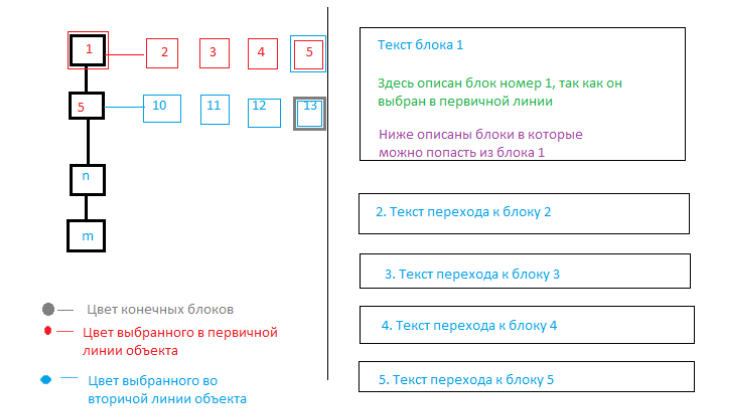
\includegraphics[width=1\linewidth]{constructor1}}
						\caption{Основной конструктор}
					\end{figure}
				\end{enumerate}
				\item Sidebar
				\begin{enumerate}
					\item Интерфейс изображенный на макете 2.
					\item Поле для ввода названия истории. (самый вверх)
					\item Кнопка «сохранить изменения».
					\item Кнопка «отменить». (После нажатия спрашивает подтверждения)
					\item Ниже кнопка «сохранить историю» (при нажатии проверяет название на предмет эквивалентности другим названиям, если название уникально, создает историю и переадресовывает на главную страницу).
					\begin{figure}[h]
						\center{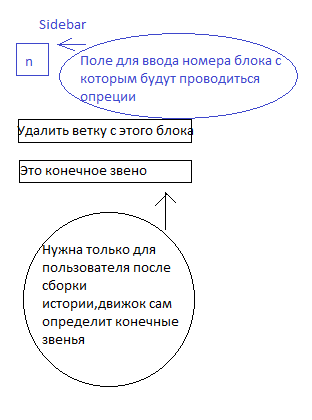
\includegraphics{constructor1_sidebar}}
						\caption{Сайдбар}
					\end{figure}
				\end{enumerate}
				\item Footer
			\end{enumerate}
			\large{Сценарии:}
				\begin{enumerate}
					\item Возможность создать историю с разветвленным сюжетом.
					\item Возможность создать обычную историю (в случае, если заполнен только первый блок).
					\item Возможность отредактировать историю (так как при нажатии кнопки «редактировать историю» открывается эта страница)
				\end{enumerate}
		\newpage
		\subsection{ID6 – Новости}
			\begin{enumerate}
				\item Header
				\item Main
				\begin{enumerate}
					\item Поле для создания новостей. (доступно администраторам)
					\item Кнопка «создать новость».
					\item Список новостей. (под каждой есть кнопка редактировать, которая преобразовывает новость в текст в textarea и появляется кнопка сохранить изменения)
					\item Над каждой новостью есть дата публикации.
				\end{enumerate}
				\item Sidebar
				\item Footer
			\end{enumerate}
			\large{Сценарии:}
				\begin{enumerate}
					\item Возможность добавить или изменить новость. (только для администраторов)
				\end{enumerate}
		\newpage
		\subsection{ID7 – «мини-форум»}
			\begin{enumerate}
				\item Header
				\item Main
				\begin{enumerate}
					\item Название выбранной темы обсуждения.
					\item Строка с количеством сообщений в данной теме.
					\item Форма для написания сообщения.
					\item Кнопка для отправки набранного сообщения (при нажатии пишет сообщение ниже, оно станет доступно всем для просмотра, а форма становится пустой).
					\item Ниже есть сообщения других пользователей в них входит аватарка пользователя, никнейм, сам текс сообщения и дата написания.
					\item Под каждым сообщением есть кнопка лайка (1 человек может поставить 1 лайк).
					\item Для администратора под каждым сообщением есть кнопка «удалить».
				\end{enumerate}
				\item Sidebar
					\begin{enumerate}
						\item Выбор темы обсуждения.
					\end{enumerate}
				\item Footer
			\end{enumerate}
			\large{Сценарии:}
				\begin{enumerate}
					\item Возможность оставить свое сообщение, в обсуждении.
					\item Возможность оценить сообщение другого человека.
				\end{enumerate}
		\newpage
		\subsection{ID8 – Правила}
			\begin{enumerate}
				\item Header
				\item Main
				\begin{enumerate}
					\item Список правил сайта
				\end{enumerate}
				\item Sidebar
				\item Footer
			\end{enumerate}
\end{document}